%=========================================================
\chapter{Modelo de negocio}
\label{cap:reqSist}

En este capítulo se describira el modelo de negocio de la aplicación SGPS referent a los puntos:
\begin{itemize}
	\item Modelo de información. En esta sección se presentan los atributos y relaciones de toda la información que contemplará el sistema.
	\item Reglas de negocio. Son las directivas destinadas a gobernar, guiar o influenciar el comportamiento de los procesos de negocio.
\end{itemize}

%------------------------------------------------------------------------------
\section{Modelo de Información: Proceso de gestión de proyectos}


\subsection{Descripción General}
En la figura \ref{fig:MOD01} se muestra la estructura de información que se manejara para el sistema de gestión de proyectos

\begin{figure}[htb]
\centering
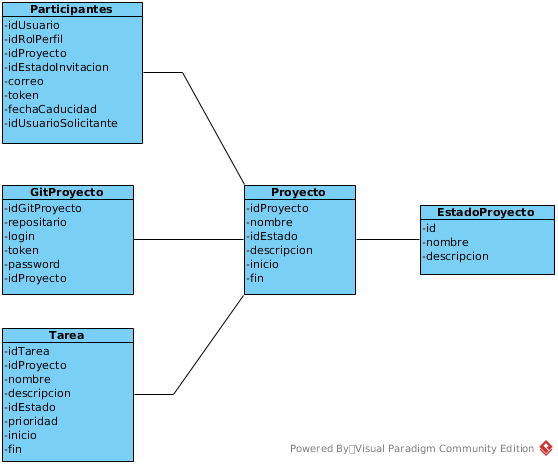
\includegraphics[width=0.8\textwidth]{./images/Modelo_Gestion_Proyectos.png}
\caption{Descripción general: Gestión de proyectos.} \label{fig:MOD01}
\end{figure}

\newpage

\subsection{Proyecto}

\begin{itemize}
	\item \textbf{Nombre} Denominación que se le da al proyecto. Es una palabra corta y este dato es requerido (no se puede omitir). Este atributo debe contener a lo mas 50 caracteres.
	\item \textbf{Descripción} Descripción de lo que trata el proyecto. Es una frase o enunciado, este dato es opcional. Este atributo debe contener a lo mas 100 caracteres.
	\item \textbf{Fecha de inicio} Fecha con la cual se indica el inicio del proyecto. Es una fecha dada en el formato dd/MMM/yyyy, este es un dato requerido (no se puede omitir).
	\item \textbf{Fecha de término} Fecha con la cual se indica el término del proyecto. Es una fecha dada en el formato dd/MMM/yyyy, este es un dato requerido (no se puede omitir).
	\item \textbf{Estado} Estado en que se encuentra el proyecto. Es dado por las diferentes situaciones en el proyecto.
\end{itemize}

\subsection{Repositorio Git}

\begin{itemize}
	\item \textbf{Repositorio} Es la URI del proyecto git que se quiere asociar con el proyecto. Es una URI la cual se obtiene desde tu repositorio git.
	\item \textbf{Token} Es una cadena la cual permite identificar al repositorio git. Es una cadena de caracteres que permite identificar si es posible conectarse al repositorio a traves de la aplicación
	\item \textbf{•}
\end{itemize}

\subsection{Participante}
\begin{itemize}
	\item \textbf{Proyecto} Es el proyecto del cual el particpante es miembro.
	\item \textbf{Estado Invitacion} Es el estado en el que se encuentra la invitacion del participante. Es dado a traves de las diferentes fases en las que se realiza el ciclo de vida de una invitación
\end{itemize}
%------------------------------------------------------------------------------
\section{Modelo de Información: Proceso de gestión de tareas}

\subsection{Descripción General}
En la figura \ref{fig:MOD02} se muestra la estructura de información que se manejara para el sistema de gestión de tareas.

\begin{figure}[htb]
\centering
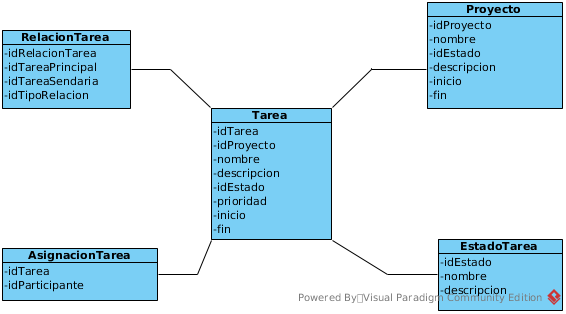
\includegraphics[width=0.8\textwidth]{./images/Modelo_Gestion_Tareas.png}
\caption{Descripción general: Gestión de tareas.} \label{fig:MOD02}
\end{figure}

\newpage

\subsection{Tarea}
\begin{itemize}
	\item \textbf{Nombre} Denominación que se le da a la tarea. Es una palabra corta y este dato es requerido (no se puede omitir). Este atributo debe contener a lo mas 150 caracteres.
	\item \textbf{Descripción} Información de lo que se tratá la tarea. Es un parrafo que describe la tarea, este es un dato opcional. Este atributo debe contener a lo mas 300 caracteres.
	\item \textbf{inicio} Fecha en la cual inicia la tarea. Es una fecha con el formato dd/MMM/yyyy, este es un dato requerido (no se puede omitir).
	\item \textbf{término} Fecha en la cual términa la tarea. Es una fecha con el formato dd/MMM/yyyy, este es un dato requerido (no se puede omitir).
\end{itemize}

\subsection{Asignacion de tarea}
\begin{itemize}
	\item \textbf{Tarea} Tarea a la cual se le asignara un participante.
	\item \textbf{Participante} Participante que se asignara a alguna tarea.
\end{itemize}

\subsection{Estado Tarea}
\begin{itemize}
	\item \textbf{Nombre} Denominación que se le da a estado de la tarea. Es una palabra corta y este dato es requerido. Este atributo puede contener a lo más 25 caracteres
	\item \textbf{Descripción} Descripción sobre el estado de la tarea. Es un parrafo de texto y este dato es obligatorio. Este atributo puede contener a lo más 25 caracteres.
\end{itemize}
%------------------------------------------------------------------------------
\section{Modelo de Información: Proceso de invitación de colaboradores}
%------------------------------------------------------------------------------
\section{Modelo de Información: Proceso de reporte de avances}